\documentclass[crop=false]{standalone}
\usepackage{standard}
\begin{document}
  \section{Methoden} % (fold)
  \label{sec:methoden}
    \subsection{Finite-Elemente-Methode} % (fold)
    \label{sub:finite_elemente_methode}

      \subsubsection{Konstruktion der schwachen Formulierung}
        Wie in Abschnitt \ref{ssub:poisson_gleichung} erwähnt, ist es bereits in der Theorie sinnvoll, die Lösungen von partiellen Differentialgleichungen in einer abgeschwächten Form zu verstehen, da bereits nicht stetige Quellterme die Forderungen an eine klassische Lösung verletzen \cite[S.~46]{Schweizer2013}.
        Demzufolge scheint eine klassische Formulierung von partiellen Differentialgleichungen für die numerische Mathematik ungeeignet.
        Für die Definition einer schwachen Lösung beziehungsweise schwachen Formulierung verallgemeinert man die Ableitung einer Funktion mithilfe von Distributionen \cite[S.~46~ff]{Schweizer2013}.
        In den Sobolevräumen werden dann die integrierbaren Funktionen zusammengefasst, die im Sinne einer Distribution wieder eine Ableitung in einem integrierbaren Raum besitzen \cite[S.~54~ff]{Schweizer2013}.

        Auf die Poisson-Gleichung wurde dieses Verfahren in Definition \ref{def:weak-formulation-poisson} bereits angewendet, sodass deren schwache Formulierung hier nicht noch einmal wiederholt werden soll.
        Allerdings wurde in den Abschnitten \ref{ssub:wellengleichung} und \ref{ssub:heat-equation} erwähnt, dass die für die Finite-Elemente-Methode benötigte schwache Formulierung der Wellen- und Wärmeleitungsgleichung durch die separate Diskretisierung der Zeit erlangt wird \cite{Alberty1998,Logan2007}.
        Es sei angemerkt, dass dies nicht die einzige Möglichkeit beschreibt, die Zeit in die Finite-Elemente-Methode einzubauen.
        Auch diese ließe sich theoretisch gesehen wie die räumlichen Dimensionen durch die Finite-Elemente-Methode behandeln.
        Dennoch erweist sich dieses Vorgehen der separaten Zeitdiskretisierung als sehr effizient sowohl bei der numerischen Behandlung als auch bei der Implementierung \cite{Logan2007}.
        Eine detailliertere Betrachtung der Theorie ist dabei in \cite[S.~211~ff]{Schweizer2013} und \cite[S.~653~ff]{Logan2007} nachzulesen.

        \paragraph{Wärmeleitungsgleichung} % (fold)
        \label{par:heat-equation}
        \hfill\\
          Für die zeitliche Diskretisierung der Wärmeleitungsgleichung kann man die sogenannte Rothe-Methode, wie sie in \cite[S.~211~ff]{Schweizer2013} und \cite{Alberty1998} beschrieben ist, verwenden.
          Sie basiert auf dem impliziten Euler-Verfahren und verhindert damit die Divergenz numerischer Lösungen \cite[S.~472~f]{Quarteroni2000}.
          Auch andere Zeitschrittverfahren, wie die Crank-Nicolson-Methode oder die Familie der Runge-Kutta-Verfahren sind jedoch denkbar \cite{Quarteroni2000,Cheney2008}.

          Es seien nun ein kleiner Zeitschritt $\infinitesimal{t}\in (0,\infty)$, ein Berechnungsgebiet $\boxBrackets{\domain} \define (\domain,\dirichletBoundary,\neumannBoundary,ν)$ und ein Wärmeleitungsproblem $(\boxBrackets{\domain},f,u_0,u^{(\mathrm{D})},u^{(\mathrm{N})},u)$ gegeben.
          Durch $\infinitesimal{t}$ wird das Zeitintervall $T\define[0,\infty)$ diskretisiert und durch die Menge $\boxBrackets{T}\define\set{k\cdot\infinitesimal{t}}{k\in\setNatural_0}$ dargestellt.
          Weiterhin bezeichne eine natürliche Zahl $n\in\setNatural$ als Index der zeitabhängigen Funktionen $f$, $u^{(\mathrm{D})}$, $u^{(\mathrm{N})}$ und $u$ deren Diskretisierung zum Zeitpunkt $n\cdot\infinitesimal{t}$.
          Dieses Schema soll am Beispiel von $u$ demonstriert werden.
          \[
            u \longleftrightarrow (u_n)_{n\in\setNatural_0}
            \separate
            u(\cdot,n\infinitesimal{t}) \longleftrightarrow u_n
          \]
          Zu beachten ist hier, dass die Diskretisierung $u_n$ im Allgemeinen $u(\cdot,n\infinitesimal{t})$ nur annähert und nicht exakt beschreibt.
          Für die Diskretisierung der zeitlichen Ableitung folgt durch die Anwendung des impliziten Euler-Verfahrens ein ähnliches Schema.
          \[
            \partial_t u \longleftrightarrow (\partial_t u_n)_{n\in\setNatural}
            \separate
            \partial_t u(\cdot,n\infinitesimal{t}) \longleftrightarrow \frac{u_{n} - u_{n-1}}{\infinitesimal{t}}
          \]
          Mit diesen Transformationen ist es jetzt möglich, die gesamte Wärmeleitungsgleichung zu diskretisieren, wie im folgenden Schema gezeigt.
          \[
            \partial_t u -\laplacian u = f
            \qquad \longleftrightarrow \qquad
            \frac{u_{n} - u_{n-1}}{\infinitesimal{t}} - \laplacian u_n = f_n
          \]
          Bei der Berechnung wird davon ausgegangen, dass $u_{n-1}$ entweder als Anfangswert $u_0$ gegeben ist oder durch einen vorherigen Zeitschritt berechnet wurde.
          Die einzige Unbekannte in der diskretisierten Gleichung ist damit $u_{n}$, für die man den folgenden Ausdruck erhält.
          \[
            \roundBrackets{\identity - \infinitesimal{t}\laplacian}u_{n} = \infinitesimal{t} f_{n} + u_{n-1}
          \]
          Für jeden Zeitpunkt $t\in\boxBrackets{T}$ handelt es sich hier um eine zeitunabhängige partielle Differentialgleichung zweiter Ordnung, deren schwache Lösung analog zu der der Poisson-Gleichung konstruiert werden kann.
          Zunächst werden die Dirichlet-Randbedingungen wieder über eine Transformation in die Gleichung eingearbeitet.
          \[
            s_n\in\setSobolev^1_\mathrm{D}(\domain)
            \separate
            s_n\define u_n - u_n^{(\mathrm{D})}
          \]
          Durch die Integration mit Testfunktionen und die Anwendung des Gaußschen Satzes erhält man nun für die schwachen Lösungen der Zeit-diskretisierten Wärmeleitungsgleichung die folgende etwas längliche Formulierung für alle $φ\in\setSobolev^1_\mathrm{D}(\domain)$.
          \begin{align*}
            &\integral{\domain}{}{s_nφ}{λ}
            + \infinitesimal{t}\integral{\domain}{}{\scalarProduct{\nabla s_n}{\nabla φ}}{λ} \\
            &= \infinitesimal{t}\boxBrackets{
              \integral{\domain}{}{f_n φ}{λ}
              + \integral{\neumannBoundary}{}{u_n^{(\mathrm{N})}φ}{σ}
              - \integral{\domain}{}{\scalarProduct{\nabla u_n^{(\mathrm{D)}}}{\nabla φ}}{λ}
            }
            \\
            &+ \integral{\domain}{}{u_{n-1} φ}{λ}
            - \integral{\domain}{}{u^{(\mathrm{D})}_{n}φ}{λ}
          \end{align*}
        % paragraph wärmeleitungsgleichung (end)

        \paragraph{Wellengleichung} % (fold)
        \label{par:wave-equation}
        \hfill\\
          Das Vorkommen der zweiten zeitlichen Ableitung in der Wellengleichung ermöglicht die Anwendung des symplektischen Euler-Verfahrens.
          Diese Methode erhält, abgesehen von kleinen Schwankungen, die Gesamtenergie eines Systems und führt damit nicht, wie beim expliziten Euler-Verfahren, zur Divergenz der Lösungen.
          Analog zur Wärmeleitungsgleichung könnte man auch hier andere Zeitschrittverfahren verwenden.

          Zunächst überführt man die Wellengleichung durch die Einführung einer neuen Variable in ein System partieller Differentialgleichungen, in der die zeitliche Ableitung nur in erster Ordnung vorkommt.
          Es seien also $\boxBrackets{\domain} \define (\domain,\dirichletBoundary,\neumannBoundary,ν)$ ein Berechnungsgebiet und $(\boxBrackets{\domain},f,φ_0, ϑ_0,φ^{(\mathrm{D})},φ^{(\mathrm{N})},φ)$ ein Wellenproblem.
          In diesem Falle gilt die folgende Äquivalenz für $ϑ\define \partial_t φ$.
          \[
            \partial_t^2 φ - \laplacian φ = f
            \qquad\iff\qquad
            \begin{pmatrix}
              \partial_t φ \\ \partial_t ϑ
            \end{pmatrix}
            =
            \begin{pmatrix}
              ϑ \\ \laplacian φ + f
            \end{pmatrix}
          \]
          Des Weiteren gelten die folgenden für die Dirichlet-Randbedingungen wichtigen Zusammenhänge für alle $t\in T$.
          \[
            φ(\cdot,0) = φ_0
            \separate
            ϑ(\cdot,0) = ϑ_0
            \separate
            \appendValue{ϑ(\cdot,t)}{\dirichletBoundary} = \appendValue{\partial_t φ^\mathrm{(D)}(\cdot,t)}{\dirichletBoundary}
          \]
          Wie zuvor bei der Wärmeleitungsgleichung soll auch hier ein kleiner Zeitschritt $\infinitesimal{t}\in(0,\infty)$ gewählt werden, der das Zeitintervall $T$ durch $\boxBrackets{T}$ diskretisiert.
          Des Weiteren soll für ein $n\in\setNatural$ die gleiche Notation für die Diskretisierung der zeitabhängigen Funktionen $f$, $φ^\mathrm{(D)}$, $φ^\mathrm{(N)}$, $φ$ und $ϑ$ verwendet werden, deren Schema noch einmal am Beispiel von φ gezeigt werden soll.
          \[
            φ\longleftrightarrow (φ_n)_{n\in\setNatural_0}
            \separate
            φ(\cdot,n\infinitesimal{t}) \longleftrightarrow φ_n
          \]
          Für die Dirichlet-Randbedingungen von $ϑ_n$ soll auch hier ein einfaches Euler-Verfahren verwendet werden.
          Da die Randbedingungen von Vornherein bekannt sind, wäre hier auch die Wahl eines analytischen Verfahrens möglich.
          \[
            \appendValue{ϑ(\cdot,n\infinitesimal{t})}{\dirichletBoundary} = \appendValue{\partial_t φ^\mathrm{(D)}(\cdot,n\infinitesimal{t})}{\dirichletBoundary}
            \qquad \longleftrightarrow \qquad
            \appendValue{ϑ_{n}}{\dirichletBoundary} = \appendValue{\frac{φ_{n}^\mathrm{(D)} - φ_{n-1}^\mathrm{(D)}}{\infinitesimal{t}}}{\dirichletBoundary}
          \]
          Für ein solches System kann nun das symplektische Euler-Verfahren explizit notiert werden.
          Die Idee besteht darin, nicht alle Terme auf der linken Seite der Gleichung gleichzeitig zu berechnen.
          In diesem Falle wird die Funktion $ϑ_{n+1}$ als Erstes berechnet, um die Berechnung von $φ_{n+1}$ zu ermöglichen.
          \[
            \begin{pmatrix}
              \partial_t φ \\ \partial_t ϑ
            \end{pmatrix}
            =
            \begin{pmatrix}
              ϑ \\ \laplacian φ + f
            \end{pmatrix}
            \qquad \longleftrightarrow \qquad
            \frac{1}{\infinitesimal{t}}\boxBrackets{
              \begin{pmatrix}
                φ_{n+1} \\ ϑ_{n+1}
              \end{pmatrix}
              -
              \begin{pmatrix}
                φ_n \\ ϑ_n
              \end{pmatrix}
            }
            =
            \begin{pmatrix}
              ϑ_{n+1} \\ \laplacian φ_n + f_n
            \end{pmatrix}
          \]
          Umgestellt nach $φ_{n+1}$ und $ϑ_{n+1}$ erhält man nun die explizite Berechnungsformel eines Zeitschrittes.
          \[
            \begin{pmatrix}
              φ_{n+1} \\ ϑ_{n+1}
            \end{pmatrix}
            =
            \begin{pmatrix}
              φ_{n} \\ ϑ_{n}
            \end{pmatrix}
            + \infinitesimal{t}
            \begin{pmatrix}
              ϑ_{n+1} \\ \laplacian φ_{n} + f_{n}
            \end{pmatrix}
          \]
          Die Konstruktion der schwachen Formulierung erfolgt wieder analog zur Wärmeleitungsgleichung.
          Zunächst werden wieder durch Hilfsvariablen die Randbedingungen eingearbeitet.
          \begin{align*}
            φ^\circ_{n+1} &\define φ_{n+1} - φ_{n+1}^\mathrm{(D)}
            &
            φ^\circ_{n+1} &\in \setSobolev^1_\mathrm{D}(\domain)
            \\
            ϑ^\circ_{n+1} &\define ϑ_{n+1} - \appendValue{ϑ_{n+1}}{\dirichletBoundary}
            &
            ϑ^\circ_{n+1} &\in \setSobolev^1_\mathrm{D}(\domain)
          \end{align*}
          Die erste Gleichung des Systems für $φ_{n+1}$ ändert sich im Prinzip nicht, da keine räumlichen Ableitungen enthalten sind.
          Das Einsetzen der Hilfsvariablen ergibt die folgende Gleichung.
          \[
            φ^\circ_{n+1} = φ^\circ_n + \infinitesimal{t} ϑ^\circ_{n+1}
          \]
          Die Umformulierung der Gleichung für $ϑ_{n+1}$ ergibt wieder einen länglichen Ausdruck für alle $ξ\in\setSobolev^1_\mathrm{D}(\domain)$.
          \begin{align*}
            \integral{\domain}{}{ϑ^\circ_{n+1}ξ}{λ}
            &= \integral{\domain}{}{ϑ_n ξ}{λ}
            - \frac{1}{\infinitesimal{t}}
            \boxBrackets{
              \integral{\domain}{}{φ_{n+1}^\mathrm{(D)}ξ}{λ}
              -\integral{\domain}{}{φ_{n}^\mathrm{(D)}ξ}{λ}
            }\\
            &+ \infinitesimal{t}
            \boxBrackets{
              \integral{\domain}{}{f_nξ}{λ}
              + \integral{\neumannBoundary}{}{φ^{(\mathrm{N})}_n ξ}{σ}
              - \integral{\domain}{}{\scalarProduct{\nabla φ_n}{\nabla ξ}}{λ}
            }
          \end{align*}
        % paragraph wellengleichung (end)
      % paragraph schritt_1_konstruktion_der_schwachen_formulierung (end)

      \subsubsection{Diskretisierung des Berechnungsgebietes}
      \label{ssub:discretization-domain}
        Aufgrund der Funktionsweise eines Computers ist man bei numerischen Simulationen gezwungen, kontinuierliche Probleme auf die eine oder andere Art und Weise zu diskretisieren.
        In der Finite-Elemente-Methode findet diese Diskretisierung durch die Einführung von finiten Elementen statt.
        Das Berechnungsgebiet $\domain$ und dessen Rand $\boundary$ werden in ein äquivalentes System von mehreren finiten Elementen überführt.
        Dabei wird die Anzahl, der Typ und die Größe dieser Elemente durch den Modellierer festgelegt.
        Für zwei Raumdimensionen werden zumeist Dreiecke und Vierecke gewählt.
        Die Abbildungen \ref{fig:domain-example} und \ref{fig:domain-discretization} veranschaulichen dieses Vorgehen im ein- und zweidimensionalen Fall anhand schematischer Beispiele.
        Das weitere Vorgehen der nächsten Paragraphen wird am Beispiel des eindimensionalen Berechnungsgebiet aus Abbildung \ref{fig:domain-example} gezeigt werden.
        \cite{Logan2007,Alberty1998,Cheney2008,Quarteroni2000}

        \begin{figure}[h]
          \center
          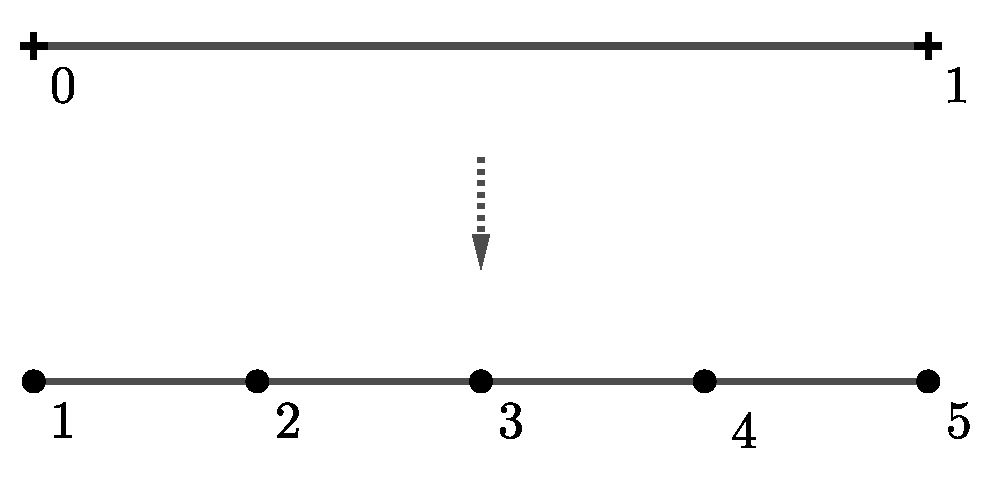
\includegraphics[width=0.5\textwidth]{images/domain_one_dimension_example.pdf}
          \caption[Diskretisierung eines eindimensionalen Berechnungsgebietes]{%
            Die Abbildung zeigt den Übergang von einem eindimensionalen Berechnungsgebiet in ein diskretisiertes Gebiet.
            Anstatt eines Intervalls wird das diskretisierte Gebiet nur noch durch Eckpunkte und deren Verbindungsstücke beschrieben.
          }
          \label{fig:domain-example}
        \end{figure}

        \begin{figure}[h]
          \begin{subfigure}[b]{0.5\textwidth}
            \center
            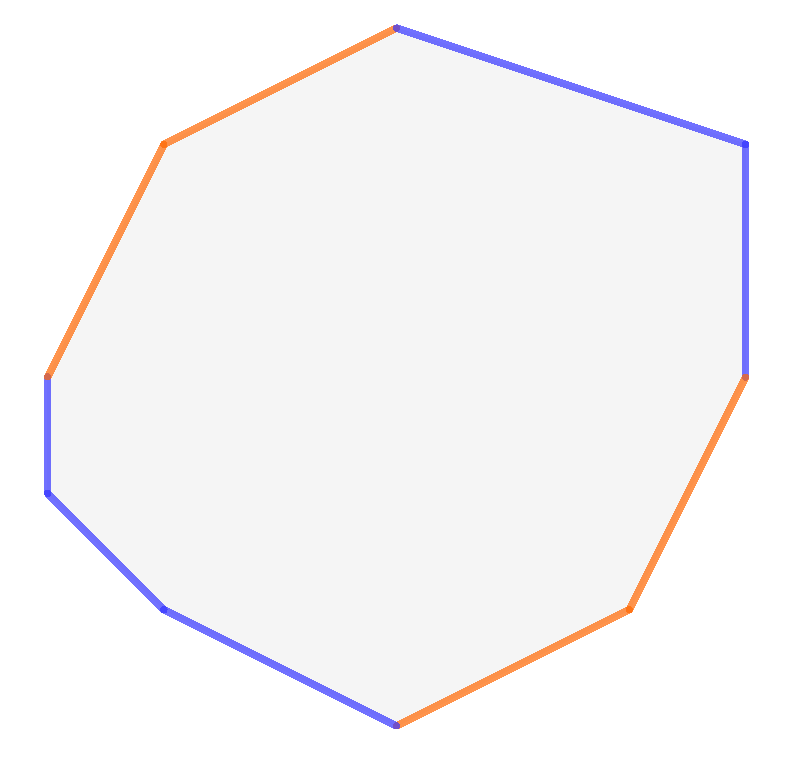
\includegraphics[width=0.6\textwidth]{images/domain_discretization_1.pdf}
          \end{subfigure}
          \begin{subfigure}[b]{0.5\textwidth}
            \center
            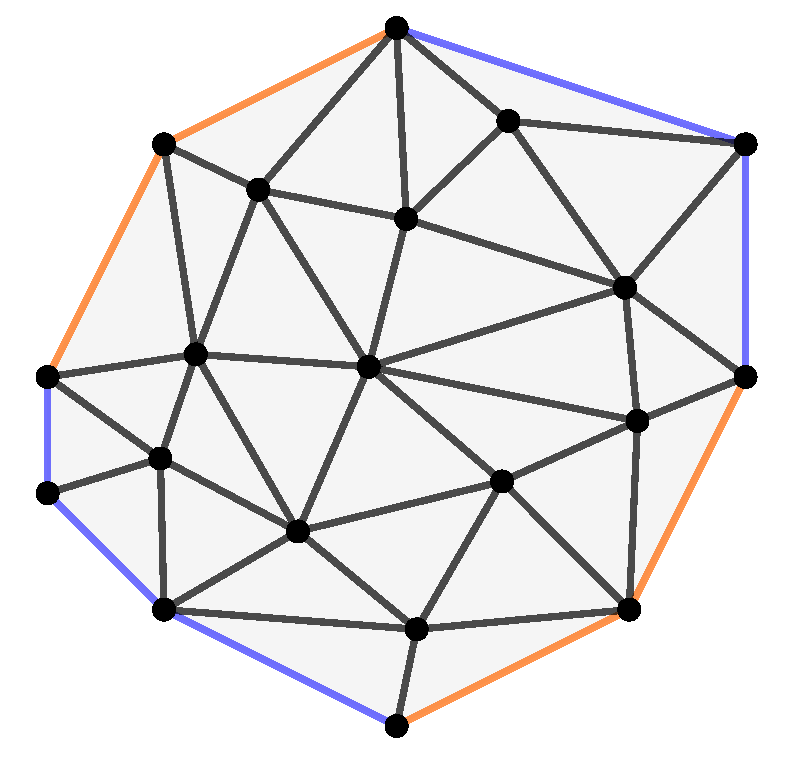
\includegraphics[width=0.6\textwidth]{images/domain_discretization_2.pdf}
          \end{subfigure}
          \caption[Diskretisierung eines zweidimensionalen Berechnungsgebietes]{%
            Die rechte Abbildung zeigt ein Beispiel für die Diskretisierung des polygonalen Berechnungsgebietes der linken Abbildung durch die Verwendung von Dreiecken.
            Die Dreiecke werden hierbei auch als finite Elemente bezeichnet.
          }
          \label{fig:domain-discretization}
        \end{figure}

        Sowohl im ein- und zweidimensionalen Fall ist zuallererst die Wahl von Eckpunkten (engl.: \textit{vertex}), die den Rand und das innere des Berechnungsgebietes näherungsweise beschreiben, nötig.
        Im Anschluss daran ist die Wahl der finiten Elemente zu treffen.
        Im eindimensionalen Beispiel aus Abbildung \ref{fig:domain-example} muss es sich dabei um Kanten handeln, die benachbarte Eckpunkte verbinden.
        Im zweidimensionalen Fall sollen in dieser Arbeit als finite Elemente nur Dreiecke gewählt werden.
        Andere Arten von finiten Elementen können vollkommen analog zu diesen eingeführt werden.
        Auch die Dreiecke definieren auf der Menge der Eckpunkte eine Art Nachbarschaft.
        Wichtig daran ist, dass sich nur die Kanten der Dreiecke schneiden dürfen, nicht aber die Dreiecke selbst, da sonst ein Teil des Berechnungsgebietes durch mehr als ein Dreieck beschrieben werden würde.

        Für den weiteren Verlauf beschreibe $V$ die endliche nichtleere Menge der gewählten Eckpunkte in einem Berechnungsgebiet.
        Um einfacher mit der Diskretisierung von Randwerten und -integralen umzugehen, soll zudem $V^\circ$ die Menge aller Eckpunkte, die nicht auf dem Dirichlet-Rand $\dirichletBoundary$ liegen, $V_\mathrm{D}$ die Menge aller Eckpunkte, die auf dem Dirichlet-Rand $\dirichletBoundary$ liegen, und $V_\mathrm{N}$ die Menge aller Eckpunkte, die auf dem Neumann-Rand $\neumannBoundary$ liegen, bezeichnen.
        In diesem Falle gelten die folgenden Beziehungen.
        \[
          V = V^\circ \cup V_\mathrm{D}
          \separate
          V^\circ \cap V_\mathrm{D} = \emptyset
          \separate
          V_\mathrm{N} \subset V^\circ
        \]
        Die Menge der Dreiecke beziehungsweise Kanten soll hier nicht weiter beschrieben werden, weil diese auch durch die Wahl der Basisfunktionen im nächsten Abschnitt gegeben ist.

        Hierfür wurde eine Menge von Dreiecken $\mathscr{T}$ gewählt, die $\bar{\domain}$ bedeckt.
        \[
          \bar{\domain} = \bigcup_{\triangle\in\mathscr{T}} \triangle
        \]
        Dies ist hier exakt möglich, da $\domain$ einen polygonalen Rand $\partial\domain$ besitzt.
        Jedes dieser Dreiecke wird durch seine drei Eckpunkte eindeutig beschrieben.

        Die Triangulierung von $\bar\domain$ ist durch einen ungerichteten Graphen $(V,E)$ beschreibbar.
        Es seien $V$ die Menge der Eckpunkte und $E$ die Menge der Kanten.
      % paragraph schritt_2_diskretisierung_des_berechnungsgebietes (end)

      \subsubsection{Wahl der Basisfunktionen}
        Neben der Diskretisierung des Berechnungsgebietes $\boxBrackets{\domain}$ ist auch die Diskretisierung der Funktionenräume $\setSobolev^1(\domain)$ und $\setSobolev^1_\mathrm{D}(\domain)$ nötig.
        Dies erreicht man durch die Wahl endlich vieler Basisfunktionen.
        Im Idealfall sollten diese einen kleinen Träger aufweisen, um die spätere Berechnung effizienter zu gestalten.
        Gerade für partielle Differentialgleichungen zweiter Ordnung ist die Wahl von stückweise linearen Basisfunktionen ausreichend, da sie, wie auch deren schwachen Lösungen, dem Raum $\setSobolev^1(\Omega)$ angehören.
        Die genannten Basisfunktion werden aufgrund ihrer Form auch Hutfunktionen genannt.
        \cite{Schweizer2013,Alberty1998,Logan2007,Cheney2008,Quarteroni2000}

        \begin{figure}
          \center
          \begin{subfigure}[b]{0.49\textwidth}
            \center
            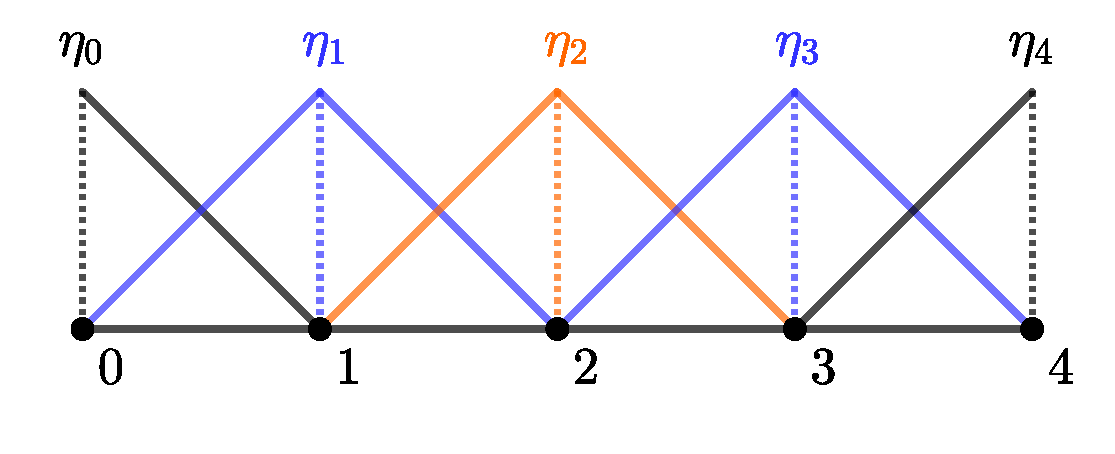
\includegraphics[width=0.95\textwidth]{images/hat_function_one_dimension_example.pdf}
          \end{subfigure}
          \begin{subfigure}[b]{0.49\textwidth}
            \center
            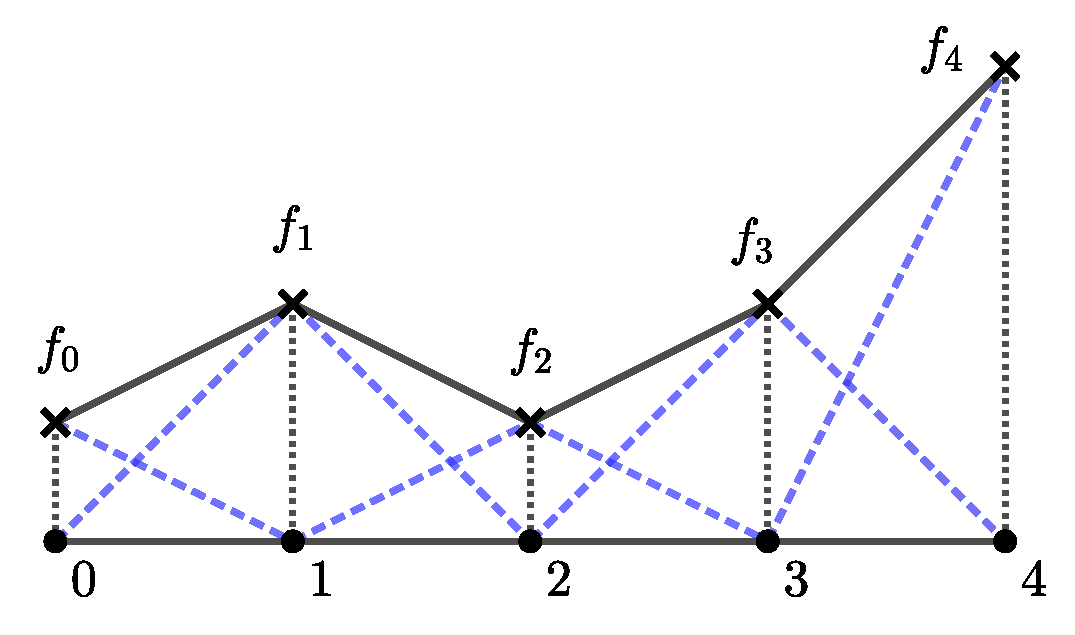
\includegraphics[width=0.95\textwidth]{images/hat_functions_linear_combination.pdf}
            \vspace{1.7mm}
          \end{subfigure}
          \caption[Eindimensionale Hutfunktionen]{%
            Die linke Abbildung zeigt die eindimensionalen Hutfunktionen $η_i$ für jeden Eckpunkt $i\in\set{0,1,2,3,4}{}$.
            Für den diskretisierten Raum von Funktionen stellen diese gerade die Basisfunktionen dar und beschreiben eine lineare Interpolation zwischen den Eckpunkten, wie sie im rechten Bild zu sehen ist.
            Die durch die Koordinaten $f_i$ beschriebene Funktion $\function{f}{[0,1]}{\setReal}$ errechnet sich zu $f(x) \define \sum_{i=0}^4 f_i η_i(x)$.
          }
          \label{fig:hat-function-example}
        \end{figure}

        \paragraph{Eindimensionale Hutfunktionen}
        \hfill\\
        Das Prinzip der Hutfunktionen soll im Folgenden am Beispiel des aus Abbildung \ref{fig:domain-example} bekannten eindimensionalen Berechnungsgebietes genauer erklärt werden.
        Abbildung \ref{fig:hat-function-example} stellt die Hutfunktionen und eine aus ihnen berechnete Beispielfunktion über dem Berechnungsgebiet schematisch dar.
        Es sei nun eine Kante $[x_i,x_j]\subset\setReal$ zwischen den aufeinanderfolgenden Eckpunkten $i\in\set{0,1,2,3}{}$ und $j=i+1$ gegeben.
        Über dieser Kante lassen sich durch eine Parametrisierung γ die stückweisen linearen Basisfunktionen leicht definieren.
        Der Definitionsbereich der Basisfunktionen ist jedoch auf die gegebene Kante eingeschränkt, um eine leichtere Handhabung zu gestatten.
        Die Gleichungen müssen für jede Kante formuliert werden.
        \[
          \function{γ}{[0,1]}{[x_i,x_j]}
          \separate
          γ(s) \define x_i (1-s) + x_j s
        \]
        \[
          \function{η_i,η_j}{[x_i,x_j]}{\setReal}
          \separate
          η_i\circ γ(s) \define 1-s
          \separate
          η_j\circ γ(s) \define s
        \]
        Bei der Parametrisierung γ handelt es sich um eine bijektive Funktion.
        Durch deren Invertierung ist eine explizite Formulierung der Basisfunktionen für alle $x\in[x_i,x_j]$ möglich.
        \[
          η_i(x) = \frac{x_j-x}{x_j-x_i}
          \separate
          η_j(x) = \frac{x-x_i}{x_j-x_i}
        \]
        Die Menge der Hutfunktionen bildet eine Basis des diskretisierten Funktionenraumes.
        Da es sich in diesem Beispiel um fünf Basisfunktionen handelt, besitzt der Funktionenraum ebenfalls die Dimension fünf.
        Jede Funktion $\function{f}{[0,1]}{\setReal}$ dieses Raums lässt sich demnach als eine Linearkombination der fünf Basisfunktionen darstellen.
        Es seien hierfür die Koordinaten $f_i\in\setReal$ für alle $i\in\set{0,1,2,3,4}{}$ gegeben.
        \[
          f = \sum_{i=0}^4 f_i η_i
        \]
        Die Bedeutung der Linearkombination für die Interpolation wird im rechten Bild von Abbildung \ref{fig:hat-function-example} gezeigt.

        \begin{figure}[h]
          \center
          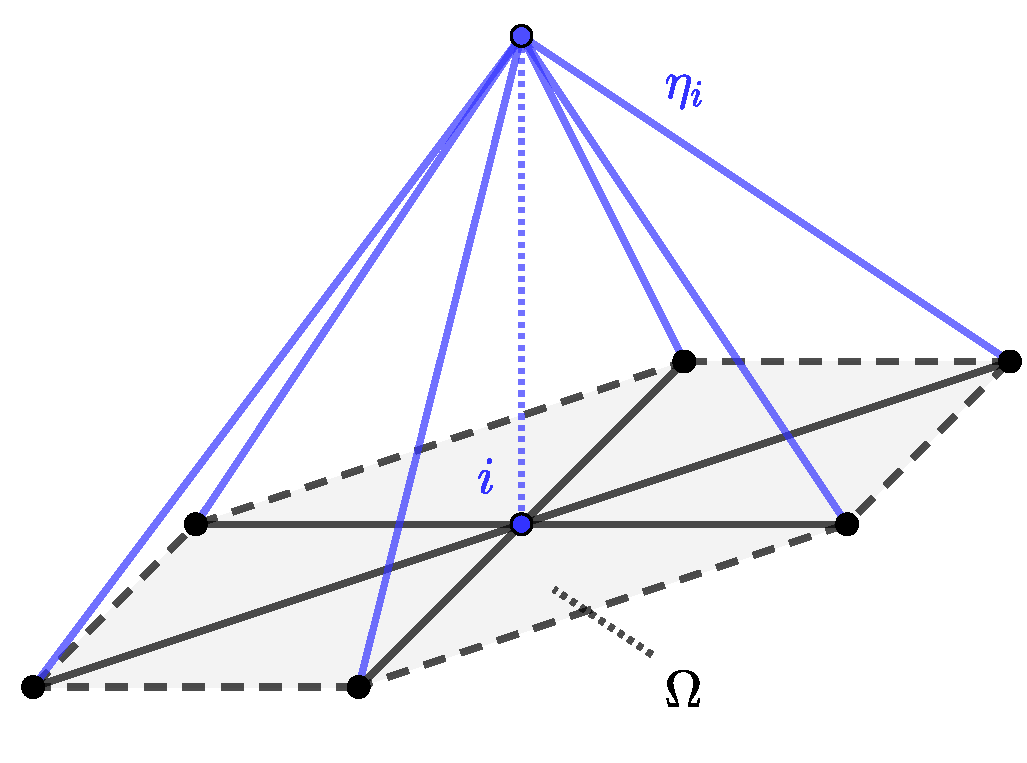
\includegraphics[width=0.5\textwidth]{images/hat_function.pdf}
          \caption[Zweidimensionale Hutfunktion]{%
            Die Abbildung zeigt die typische Wahl einer Basisfunktion $η_i$ über dem $i$.~Vertex des diskretisierten Berechnungsgebietes $\domain$.
            Aufgrund ihrer Form wird sie auch Hutfunktion genannt.
            Sie ist stückweise linear und identisch zu Null auf nicht benachbarten Dreiecken.
            Sie entspricht einer linearer Interpolation zwischen den Eckpunkten.
          }
          \label{fig:hat-function}
        \end{figure}

        \paragraph{Zweidimensionale Hutfunktionen auf dem Dreieck}
        \hfill\\
        Abbildung \ref{fig:hat-function} stellt eine zweidimensionale Hutfunktion über einem Eckpunkt des diskretisierten Berechnungsgebietes dar.
        Der Träger der Funktion ist auf benachbarte Dreiecke beschränkt.
        Außerhalb dieser Dreiecke ist die Hutfunktion identisch zu Null.
        Für die folgenden Formeln und Berechnungsschritte wurde das Vorgehen aus \cite{Alberty1998} gewählt.

        \begin{wrapfigure}{l}{0.4\textwidth}
          \center
          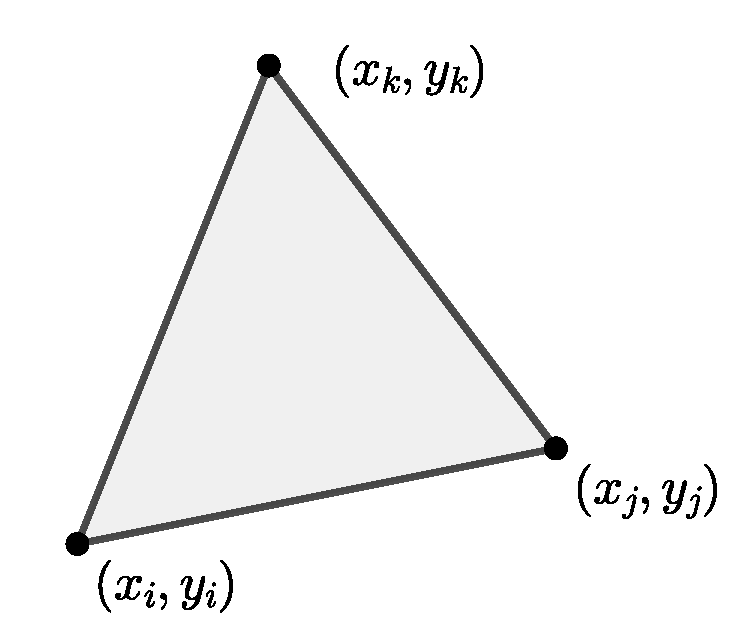
\includegraphics[width=0.4\textwidth]{images/triangle.pdf}
        \end{wrapfigure}
        Für den zweidimensionalen Fall betrachte man ein Dreieck, welches durch die Eckpunkte $(x_i,y_i)$, $(x_j,y_j)$ und $(x_k,y_k)$ aus der Menge $\setReal^2$ gegeben ist.
        Die Menge aller Punkte des Dreiecks sei definiert als $\triangle$.
        Um die Hutfunktionen auf eine einfache Weise zu definieren, konstruiert man auch für dieses Dreieck zunächst eine Parametrisierung, die auf den baryzentrischen Koordinaten basiert.
        \[
          M\define\set{(u,v)\in[0,1]^2}{u+v\leq 1}
        \]
        $M$ dient hier als der Definitionsbereich dieser Parametrisierung.
        Die Hutfunktionen seien hier mit $η_i$, $η_j$ und $η_k$ bezeichnet.
        Zu beachten ist dabei, dass der Definitionsbereich der Basisfunktionen wieder auf das zugrundeliegende Dreieck eingeschränkt ist.
        Die Gleichungen müssen also auch hier für jedes Dreieck des diskretisierten Berechnungsgebietes formuliert werden.
        \[
          \function{γ}{M}{\triangle}
          \separate
          γ(u,v) \define
          (1-u-v)
          \begin{pmatrix}
            x_i \\ y_i
          \end{pmatrix}
          + u
          \begin{pmatrix}
            x_j \\ y_j
          \end{pmatrix}
          + v
          \begin{pmatrix}
            x_k \\ y_k
          \end{pmatrix}
        \]
        \[
          \function{η_i,η_j,η_k}{\triangle}{\setReal}
        \]
        \[
          η_i\circ γ(u,v) \define 1-u-v
          \separate
          η_j\circ γ(u,v) \define u
          \separate
          η_k\circ γ(u,v) \define v
        \]
        Um nun die Basisfunktionen in expliziter Form zu erhalten, muss die bijektive Parametrisierung γ invertiert werden.
        Dies geschieht durch ein lineares Gleichungssystem, welches auf dem Papier durch ein analytisches Verfahren leicht aufgelöst werden kann.
        Die genauen Rechnungen sollen hier aus Platzgründen nicht vorgeführt werden.
        Man erhält damit für alle $(x,y)\in\triangle$ die folgenden Ausdrücke.
        \begin{align*}
          η_i(x,y) &= \frac{1}{α}
          \begin{vmatrix}
            1 & x & y \\
            1 & x_j & y_j \\
            1 & x_k & y_k
          \end{vmatrix}
          &
          η_j(x,y) &= \frac{1}{α}
          \begin{vmatrix}
            1 & x & y \\
            1 & x_k & y_k \\
            1 & x_i & y_i
          \end{vmatrix}
          \\
          η_k(x,y) &= \frac{1}{α}
          \begin{vmatrix}
            1 & x & y \\
            1 & x_i & y_i \\
            1 & x_j & y_j
          \end{vmatrix}
          &
          α &\define
          \begin{vmatrix}
            1 & x_i & y_i \\
            1 & x_j & y_j \\
            1 & x_k & y_k
          \end{vmatrix}
        \end{align*}
        Wie auch im eindimensionalen Fall wird der diskretisierte Funktionenraum $\mathrm{S}$ durch die Menge der Linearkombination der Basisfunktionen beschrieben.
        Es sei dabei $V$ wieder die Menge aller Eckpunkte des diskretisierten Berechnungsgebietes.
        \[
          \mathrm{S} \define \mathrm{span}\set{η_i}{i\in V} \subset \setSobolev^1(\domain)
          \separate
          \mathrm{S}_\mathrm{D} \define \mathrm{S} \cap \setSobolev^1_\mathrm{D}(\domain)
        \]
      % paragraph schritt_3_wahl_der_basisfunktionen (end)

      \subsubsection{Konstruktion der algebraischen Formulierung}
        Nachdem sowohl das Berechnungsgebiet als auch die Funktionenräume diskretisiert wurden, ist es nun möglich, darauf aufbauend aus den schwachen Formulierungen der partiellen Differentialgleichungen ein System algebraischer Gleichungen zu erlangen.
        Grundsätzlich ersetzt das Vorgehen alle Funktionen aus den Räumen $\setSobolev^1_\mathrm{D}(\domain)$ und $\setSobolev^1(\domain)$ durch die stückweisen linearen Funktionen der Räume $\mathrm{S}_\mathrm{D}$ und $\mathrm{S}$.
        Das Verfahren soll zunächst anhand des Poisson-Problems demonstriert werden.
        Das resultierende lineare Gleichungssystem lässt sich dann analog auch für das Wellen- und Wärmeleitungsproblem herleiten.

        \paragraph{Poisson-Problem} % (fold)
        \hfill\\
          Es sei wieder $([\Omega], f, u^\mathrm{(D)}, u^\mathrm{(N)},u)$ ein Poisson-Problem.
          Nach Definition \ref{def:weak-formulation-poisson} ist die schwache Formulierung des Poisson-Problems durch die folgende Gleichung für alle $φ\in\setSobolev^1_\mathrm{D}(\domain)$ gegeben.
          \[
            \integral{\domain}{}{\scalarProduct{\nabla v}{\nabla φ}}{λ} = \integral{\domain}{}{f φ}{λ} + \integral{\neumannBoundary}{}{u^\mathrm{(N)} φ}{σ} - \integral{\domain}{}{\scalarProduct{\nabla u^\mathrm{(D)}}{\nabla φ}}{λ}
          \]
          Weiterhin sei die Menge der Eckpunkte des diskretisierten Berechnungsgebietes durch $V$ und deren zugehörige Basisfunktionen durch die Menge $B\define\set{\function{η_i}{\domain}{\setReal}}{i\in V}$ gegeben.
          Um die Notation etwas leichter zu gestalten, werden die folgenden natürlichen Zahlen eingeführt.
          \[
            n\define \absolute{V}
            \separate
            m\define \absolute{V^\circ}
            \separate
            p\define \absolute{V_\mathrm{D}}
            \separate
            q\define \absolute{V_\mathrm{N}}
          \]
          Alle Funktionen des Poisson-Problems sollen nun durch den diskreten Raum der Funktionen beschrieben werden.
          Hierfür wählt man die folgenden Vektoren $\boxBrackets{f},\boxBrackets{u}\in\setReal^n$, $\boxBrackets{u^\mathrm{(D)}}\in \setReal^p$, $\boxBrackets{u^\mathrm{(N)}} \in \setReal^q$, $\boxBrackets{v}\in \setReal^m$.
          Diese Vektoren beschreiben die Koordinaten bezüglich der gewählten Basisfunktionen.
          \begin{align*}
            f &= \sum_{i\in V} \boxBrackets{f}_i η_i
            &
            u^\mathrm{(D)} &= \sum_{i\in V_\mathrm{D}} \boxBrackets{u^\mathrm{(D)}}_i η_i
            \\
            v &= \sum_{i\in V^\circ} \boxBrackets{v}_i η_i
            &
            u^\mathrm{(N)} &= \sum_{i\in V_\mathrm{N}} \boxBrackets{u^\mathrm{(N)}}_i \appendValue{η_i}{\neumannBoundary}
          \end{align*}
          \[
            u
            = \sum_{i\in V} \boxBrackets{u}_i η_i
            = \underbrace{\sum_{i\in V^\circ} \boxBrackets{v}_i η_i}_{= v}
            + \underbrace{\sum_{i\in V_\mathrm{D}} \boxBrackets{u^\mathrm{(D)}}_i η_i}_{=u^\mathrm{(D)}}
            = v + u^\mathrm{(D)}
          \]
          Diese verschiedenen Ausdrücke werden nun in das Poisson-Problem eingesetzt.
          In der schwachen Formulierung des Poisson-Problems kann das $φ\in\setSobolev^1_\mathrm{D}(\domain)$ direkt durch alle Basisfunktionen ersetzt werden.
          Man erhält damit für alle $i\in V^\circ$ die folgende Gleichung.
          \begin{align*}
            \sum_{j\in V^\circ} u_j \integral{\domain}{}{\scalarProduct{\nabla η_i}{\nabla η_j}}{λ}
            &= \sum_{j \in V} f_j \integral{\domain}{}{η_iη_j}{λ}
            + \sum_{j \in V_\mathrm{N}} u_j^\mathrm{(N)} \integral{\neumannBoundary}{}{η_i η_j}{σ}
            \\
            &- \sum_{j \in V_\mathrm{D}} u_j^\mathrm{(D)} \integral{\domain}{}{\scalarProduct{\nabla η_i}{\nabla η_j}}{λ}
          \end{align*}
          Fasst man dies zu einem System von Gleichungen zusammen, so entsteht ein lineares Gleichungssystem.
          Für eine einfachere Notation führt man aus diesem Grund die Matrizen $\boxBrackets{\laplacian}\in\setReal^{m\times m}$, $\boxBrackets{M}\in\setReal^{m\times n}$, $\boxBrackets{N}\in\setReal^{m\times q}$ und $\boxBrackets{D}\in\setReal^{m\times p}$ ein.
          \begin{align*}
            \boxBrackets{\laplacian}_{ij} &\define \integral{\domain}{}{\scalarProduct{\nabla η_i}{\nabla η_j}}{λ}
            &
            \boxBrackets{M}_{ij} &\define \integral{\domain}{}{η_iη_j}{λ}
            \\
            \boxBrackets{D}_{ij} &\define \integral{\domain}{}{\scalarProduct{\nabla η_i}{\nabla η_j}}{λ}
            &
            \boxBrackets{N}_{ij} &\define \integral{\neumannBoundary}{}{η_iη_j}{σ}
          \end{align*}
          Die Matrix $\boxBrackets{\laplacian}$ wird auch \enquote{Stiffness Matrix} und $\boxBrackets{M}$ auch \enquote{Mass Matrix} genannt.
          In der einfacheren Matrix-Vektor-Notation lässt sich das System linearer Gleichungen nun wie folgt schreiben.
          \[
            [\laplacian][v] = [M][f] + [N][u^\mathrm{(N)}] - [\laplacian][u^\mathrm{(D)}]
          \]
          Bei $[\laplacian]$ handelt es sich um eine symmetrische, positiv-definite Matrix \cite{Alberty1998}.
          Für das System linearer Gleichungen existiert damit eine eindeutige Lösung.

          Ein letzter Schritt für die Formulierung des linearen Gleichungssystems kümmert sich nun darum, die komplexen Systemmatrizen aus den einfachen Matrizen der finiten Elemente zu konstruieren.
          Es sei $\mathscr{T}$ die Menge der finiten Elemente, die das Berechnungsgebiet diskretisieren.
          Das Integral über $\domain$ lässt sich für eine beliebige Funktion damit als Summe der Integrale über die finiten Elemente darstellen.
          \[
            \integral{\domain}{}{η_iη_j}{λ} = \sum_{E\in\mathscr{T}} \integral{E}{}{η_iη_j}{λ}
            \separate
            \integral{\domain}{}{\scalarProduct{\nabla η_i}{\nabla η_j}}{λ} = \sum_{E\in\mathscr{T}} \integral{E}{}{\scalarProduct{\nabla η_i}{\nabla η_j}}{λ}
          \]
          Durch die kleinen Träger der Basisfunktionen sind die beschriebenen Integrale häufig Null.
          Wählt man demnach zwei Basisfunktionen $η_i$ und $η_j$, deren Eckpunkte $i$ und $j$ nicht durch die Kante eines finiten Elements verbunden sind, so ergibt sich das Folgende für alle $E\in\mathscr{T}$.
          \[
            \integral{E}{}{η_iη_j}{λ} = \integral{\domain}{}{η_iη_j}{λ} = 0
            \separate
            \integral{E}{}{\scalarProduct{\nabla η_i}{\nabla η_j}}{λ} = \integral{\domain}{}{\scalarProduct{\nabla η_i}{\nabla η_j}}{λ} = 0
          \]
          Ein ähnliches Vorgehen kann auch für die Integrale über dem Rand $\neumannBoundary$ gewählt werden.
          Die komplexen Systemmatrizen ergeben sich damit als eine Summe von einfach zu beschreibenden Finite-Elemente-Matrizen.
        % paragraph poisson_problem_am_eindimensionalen_beispiel (end)

        \paragraph{Eindimensionales Beispiel des Poisson-Problems} % (fold)
        \label{par:eindimensionales_beispiel}
        \hfill\\
          Das lineare Gleichungssystem soll einmal für das eindimensionale Beispiel aus Abbildung \ref{fig:domain-example} notiert werden.
          Dabei sollen an den Randpunkten Dirichlet-Randbedingungen herrschen.
          Die Neumann-Randbedingungen werden also für dieses Beispiel vernachlässigt.
          Als Erstes werden die einfachen Matrizen jeder einzelnen Kante $[x_i,x_j]$ mit $i\in\set{0,1,2,3}{}$ und $j=i+1$ konstruiert.
          Die Länge aller Kanten ist gleich und soll als $h\define x_j-x_i$ bezeichnet werden.
          \[
            \roundBrackets{ \integral{[x_i,x_j]}{}{η_pη_q}{λ} }_{p,q\in\set{i,j}{}}
            = \frac{h}{6}
            \begin{pmatrix}
              2 & 1 \\
              1 & 2
            \end{pmatrix}
          \]
          \[
            \roundBrackets{ \integral{[x_i,x_j]}{}{\scalarProduct{\nabla η_p}{\nabla η_q}}{λ} }_{p,q\in\set{i,j}{}}
            = \frac{1}{h}
            \begin{pmatrix}
              1 & -1 \\
              -1 & 1
            \end{pmatrix}
          \]
          Die Addition der einzelnen Finite-Elemente-Matrizen jeder Kanten ergibt dann die komplette Stiffness und Mass Matrix.
          \[
            \roundBrackets{ \integral{\domain}{}{η_i η_j}{λ} }_{i\in V^\circ,j\in V} = \frac{h}{6}
            \begin{pmatrix}
              1 & 4 & 1 & & \\
              & 1 & 4 & 1 & \\
              & & 1 & 4 & 1 \\
            \end{pmatrix}
          \]
          \[
            \roundBrackets{ \integral{\domain}{}{ \scalarProduct{\nabla η_i}{\nabla η_j} }{λ} }_{i,j\in V^\circ} = \frac{1}{h}
            \begin{pmatrix}
              2 & -1 & \\
              -1 & 2 & -1 \\
              & -1 & 2 \\
            \end{pmatrix}
          \]
          \[
            \roundBrackets{ \integral{\domain}{}{ \scalarProduct{\nabla η_i}{\nabla η_j} }{λ} }_{i\in V^\circ,j\in V_\mathrm{D}} = \frac{1}{h}
            \begin{pmatrix}
              -1 & 0 \\
              0 & 0 \\
              0 & -1 \\
            \end{pmatrix}
          \]
          Diese setzt man nun in die Gesamtgleichung ein und erhält das folgende Gleichungssystem, welches nach $[v]$ aufgelöst werden soll.
          \[
            \frac{1}{h}
            \begin{pmatrix}
              2 & -1 & \\
              -1 & 2 & -1 \\
              & -1 & 2 \\
            \end{pmatrix}
            \begin{pmatrix}
              v_1 \\ v_2 \\ v_3
            \end{pmatrix}
            =
            \frac{h}{6}
            \begin{pmatrix}
              1 & 4 & 1 & & \\
              & 1 & 4 & 1 & \\
              & & 1 & 4 & 1 \\
            \end{pmatrix}
            \begin{pmatrix}
              f_0 \\ f_1 \\ f_2 \\ f_3 \\ f_4
            \end{pmatrix}
            -
            \frac{1}{h}
            \begin{pmatrix}
              -1 & 0 \\
              0 & 0 \\
              0 & -1 \\
            \end{pmatrix}
            \begin{pmatrix}
              u^\mathrm{(D)}_0 \\ u^\mathrm{(D)} _4
            \end{pmatrix}
          \]
        % paragraph eindimensionales_beispiel (end)

        \paragraph{Konstruktion der Matrizen im Zweidimensionalen} % (fold)
        \label{par:konstruktion_der_matrizen_im_zweidimensionalen}
          \[
            \roundBrackets{ \integral{\triangle}{}{η_pη_q}{λ} }_{p,q\in\set{i,j,k}{}}
            = \frac{λ(\triangle)}{12}
            \begin{pmatrix}
              2 & 1 & 1 \\
              1 & 2 & 1 \\
              1 & 1 & 2
            \end{pmatrix}
          \]
          \[
            \roundBrackets{ \integral{\triangle}{}{\scalarProduct{\nabla η_p}{\nabla η_q}}{λ} }_{p,q\in\set{i,j,k}{}}
            = \frac{1}{4λ(\triangle)} \transpose{D}D
          \]
          \[
            D \define
            \begin{pmatrix}
              x_k-x_j & x_i-x_k & x_j-x_i \\
              y_k-y_j & y_i-y_k & y_j-y_i
            \end{pmatrix}
          \]
          \[
            \roundBrackets{ \integral{E}{}{η_pη_q}{σ} }_{p,q\in\set{i,j}{}}
            = \frac{σ(E)}{6}
            \begin{pmatrix}
              2 & 1 \\
              1 & 2
            \end{pmatrix}
          \]
        % paragraph konstruktion_der_matrizen_im_zweidimensionalen (end)
      % paragraph schritt_4_konstruktion_der_algebraischen_formulierung (end)

      \subsubsection{Lösung des algebraischen Systems}
        Die erhaltenen algebraischen Gleichungen sind äquivalent zu der schwachen Formulierung des diskretisierten Problems.
        In den hier betrachteten Fällen existieren eindeutige Lösungen.

        Das Einsetzen der Diskretisierung in die ursprüngliche schwache Formulierung der partiellen Differentialgleichung führt zu einem System von algebraischen Gleichungen.
        Die in dieser Arbeit besprochenen Fälle resultieren in linearen Gleichungssystemen mit dünnbesetzten Matrizen.
        Diese hängen zudem stark von der gewählten Diskretisierung ab.
      % paragraph schritt_5_lösen_des_algebraischen_systems (end)

    % subsection finite_elemente_methode (end)

    \subsection{Numerische Methoden dünnbesetzter Matrizen} % (fold)
    \label{sub:sparse_matrix_methoden}
      Dünnbesetzte Matrizen (engl.: \textit{sparse matrix}) treten in einem beträchtlichen Anteil numerischer Disziplinen auf und als ein Resultat sind Methoden, um diese effizient zu manipulieren, häufig ein kritischer Punkt der Performance vieler Anwendungen.
      Vor allem die Matrix-Vektor-Multiplikation dünnbesetzter Systeme repräsentiert zumeist die dominanten Kosten vieler iterativer Lösungsmethoden linearer Systeme großen Ausmaßes \cite{Bell2008}.
      Gerade bei der Finite-Elemente-Methode werden Mass und Stiffness Matrix im Computer durch ein Sparse-Matrix-Format dargestellt \cite{Bell2008,Logan2007,Alberty1998}.
      Die Wahl der Speicherformate und Lösungsmethoden wirken sich dabei extrem auf die Performance der Anwendung aus \cite{Bell2008,Bell2009}.

      \subsubsection{Datenstrukturen und das CSR-Format} % (fold)
      \label{ssub:datenstrukturen_und_speicherformate}
        Eine Sparse-Matrix $M\in\setReal^{n\times n}$ mit $n\in\setNatural$, deren Anzahl von Elementen ungleich Null der Größenordnung $n$ entspricht, kann durch das Allozieren aller $n^2$ Speicherplätze nicht effizient dargestellt werden.
        Häufig stellt dieses Unterfangen sogar eine physikalische Unmöglichkeit dar, weil ab einer bestimmten Größe von $n$ der Speicherplatz für die $n^2$ Elemente nicht einmal existiert.
        Selbst wenn man den Speicher allozieren könnte, so wäre eine Iteration über alle Elemente, eine häufige Operation bei der Verwendung von Matrizen, reine Zeitverschwendung, da ein Großteil dieser Elemente Null wäre.
        Offensichtlich müssen also gewisse indizierte Speicherschemen verwendet werden, um die Natur einer dünnbesetzten Matrix effizient zu beschreiben.
        \cite[S.~78]{Press2002}

        Typische Datenstukturen für die Verwendung dünnbesetzter Matrizen werden durch die Formate COO (engl.: \textit{coordinate list}), CSR (engl.: \textit{compressed sparse row}) und ELLPACK (ELL) dargestellt \cite{Bell2008,Bell2009}.
        Allerdings existieren wesentlich mehr Formate, die im Rahmen dieser Arbeit nicht erwähnt werden können.
        Untersuchungen über die Implementierung der genannten Formate auf der GPU sind in \cite{Bell2008} und \cite{Bell2009} zu finden.
        Jedes Format besitzt Vor- und Nachteile.
        Bis auf das COO-Format scheint die Effizienz zudem vom genauen Muster der dünnbesetzten Matrix abzuhängen.
        Es stellte sich heraus, dass das CSR-Format eine sehr gute durchschnittliche Performance ermöglicht.
        Aus diesem Grund beschränkt sich diese Arbeit auf die Beschreibung und Implementierung dessen.
        Eine genauere Erläuterung des ELL-Formates ist im Anhang zu finden.

        Für eine Matrix $M\in\setReal^{n\times n}$ mit $k\in\setNatural,k\leq n^2$ Einträgen ungleich Null speichert das CSR-Format diese in einem Tupel $\boxBrackets{M}_\mathrm{CSR}$ dreier Vektoren.
        \[
          \boxBrackets{M}_\mathrm{CSR} \define (V,R,C)
          \separate
          V \in \setReal^{k}
          \separate
          R \in \setNatural_0^{n+1}
          \separate
          C \in \setNatural_0^{k}
        \]
        In $V$ werden dabei alle Werte ungleich Null gespeichert, indem Zeile für Zeile alle Spalten von links nach rechts ausgelesen werden.
        Dies bedeutet, dass alle Werte $a_{ij}$ von $M$ mit $(i,j)\in\setNatural^2$ und $i,j\leq n$, die ungleich Null sind, anhand von $m(i-1,j-1)$ geordnet werden.
        \[
          \function{m}{\set{p\in\setNatural_0}{p< n}^2}{\setNatural_0}
          \separate
          m(i,j) \define n\cdot i + j
        \]
        Für jedes $i\in\setNatural$ mit $i\leq n+1$ speichert $R_{i}$ die Anzahl der Werte ungleich Null, die bis zur Zeile $i$ von $M$ vorkommen.
        $R_0$ wird dabei immer auf Null gesetzt.
        Demnach kann $R$ als kumulative Verteilungsfunktion der Einträge ungleich Null über die Zeilen verstanden werden.
        In $C$ werden die Spaltenindizes eines jeden Wertes aus $V$ gespeichert.
        Dieses Vorgehen soll an dem folgenden Beispiel gezeigt werden \cite{Eigen2018}.
        \[
          M =
          \begin{pmatrix}
            0 & 3 & 0 & 0 & 0 \\
            22 & 0 & 0 & 0 & 17 \\
            7 & 5 & 0 & 1 & 0 \\
            0 & 0 & 0 & 0 & 0 \\
            0 & 0 & 14 & 0 & 8
          \end{pmatrix}
          \separate
          \boxBrackets{M}_\mathrm{CSR} = \roundBrackets{
            \begin{pmatrix}
              3 \\ 22 \\ 17 \\ 7 \\ 5 \\ 1 \\ 14 \\ 8
            \end{pmatrix},
            \begin{pmatrix}
              0 \\ 1 \\ 3 \\ 6 \\ 6 \\ 8
            \end{pmatrix},
            \begin{pmatrix}
              1 \\ 0 \\ 4 \\ 0 \\ 1 \\ 3 \\ 2 \\ 4
            \end{pmatrix}
          }
        \]

        Für Berechnung des Matrix-Vektor-Produktes eines Vektors $x\in\setReal^n$ mit der Matrix $M \reverseDefine (a_{ij})_{i,j}$, gespeichert durch $[M]_\mathrm{CSR}$, wird im einfachsten Fall zunächst zeilenweise gearbeitet.
        Für jede Zeile $i\in\setNatural$ mit $i\leq n$ muss ein einfaches Skalarprodukt ausgewertet werden.
        \[
          \roundBrackets{Mx}_i = \sum_{j=1}^n a_{ij} x_j = \sum_{j=R_i+1}^{R_{i+1}} V_j x_{C_{j}+1} = \roundBrackets{[M]_\mathrm{CSR}x}_i
        \]

        Ein analoges Verfahren ist das sogenannten CSC-Format (engl.: \textit{compressed sparse column}).
        Hier wird die kumulative Verteilungsfunktion im Bezug auf die Spalten und nicht auf die Zeilen gebildet.
        \cite{Bell2008}



        \paragraph{Vergleich der Anwendbarkeit} % (fold)
        \label{par:vergleich_der_anwendbarkeit}
          \begin{figure}[h]
            \center
            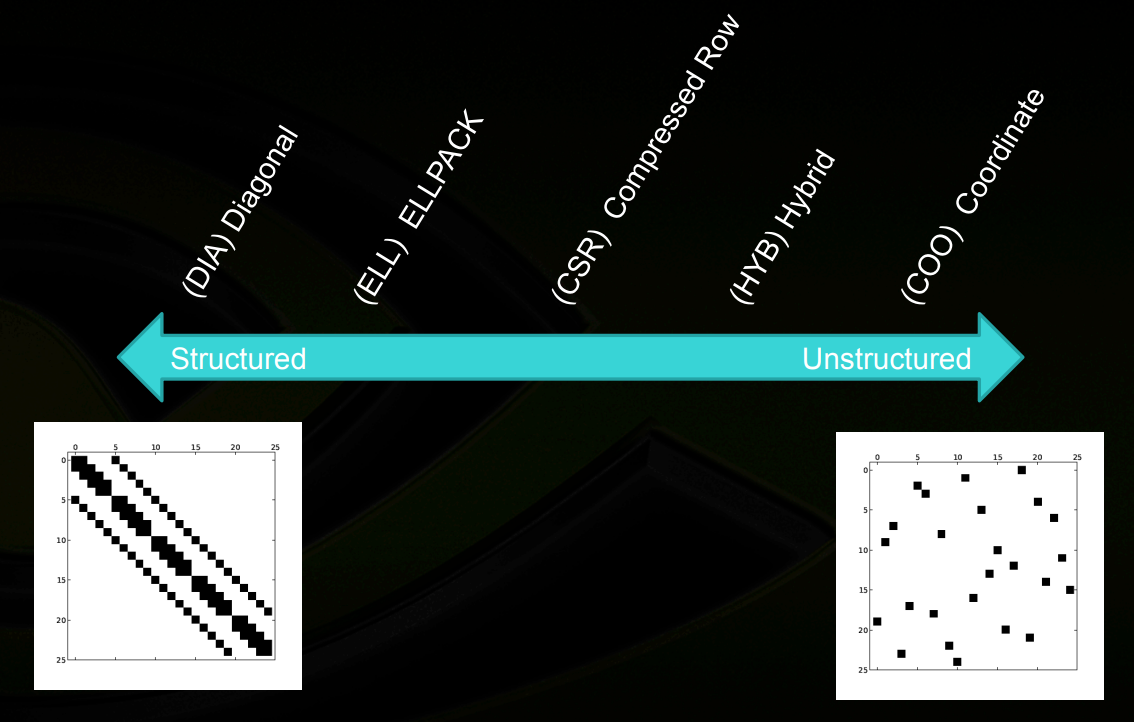
\includegraphics[width=0.8\textwidth]{images/comparison_sparse_matrix_formats.png}
          \end{figure}
        % paragraph vergleich_der_anwendbarkeit (end)
      % subsubsection datenstrukturen_und_speicherformate (end)

      \subsubsection{Assemblierung dünnbesetzter Matrizen} % (fold)
      \label{ssub:assemblierung_dünnbesetzter_matrizen}

      % subsubsection assemblierung_dünnbesetzter_matrizen (end)

      \subsubsection{Lösung dünnbesetzter Systeme} % (fold)
      \label{ssub:lösung_dünnbesetzter_systeme}
        \cite[S.~101~ff]{Nocedal2006}
      % subsubsection lösung_dünnbesetzter_systeme (end)
    % subsection sparse_matrix_methoden (end)
  % section methoden (end)
\end{document}